\chapter{Teoretický základ}
\label{sec:te}

\section{Základní pojmy}

\begin{itemize}
    \item client/server
    \item tcp/ip
    \item osi
    \item mqtt
    \item certifikát, k~tomu veřejný a soukromý klíč, self-signed jen treba lehce zminit, protoze je uz dost popsanej v~ty http sekci
    \item vícevláknová obsluha
    \item csrf, mozna xss sqlinjection
    \item publisher/subscriber
    \item webové rozhraní
    \item unix time
    \item cloud
    \item relacni databaze, databazovy schema, vztahy (1:n, atd)
    \item navrhovy vzory -- mvc
\end{itemize}

\section{Protokol HTTP}

\subsection{Požadavek}
% u pozadavku popsat navratovy kod, metody, hlavicku

\subsection{Relace}

\section{Nadřazený systém}

Zařízení, jehož tvorba je cílem práce, je v~textu označováno jako nadřazený systém. Podrobná specifikace nadřazeného systému je popsána v~úvodu kapitoly \ref{sec:an}.

\section{Podřízený systém}

Podřízené systémy jsou monitorovací zařízení, která jsou umístěná v~jednotlivých garážích. Zařízení neoperují samostatně, ale zasílají data nadřazenému systému. Podřízený systém je blíže popsán v~sekci \ref{sec:an_subsystem}.

\section{Uživatel}

Uživatelem se v~textu práce myslí osoba spravující nadřazený systém a přistupující do jeho webového rozhraní. Jde tedy například o~majitele garáží nebo zaměstnance pověřeného jejich správou.

% \section{API} to mozna necham jen ve zkratkach, stejne tak JSON

\section{Klíč}

Náhodně generovaná data (například ve formě textového řetězce), která slouží k~ověření totožnosti. Znalost klíče umožní přístup k~šifrovaným datům nebo jinak zakázaným operacím. V~této práci se hovoří většinou o~API klíčích, kterými se prokazují podřízené systémy při komunikaci s~nadřazeným systémem.

\section{\textit{Attack surface}}

\textit{Attack surface} popisuje všechny možné body, kde by mohl potencionální útočník napadnout daný systém \cite{attack_surface_owasp}. V~této práci je zmíněn v~sekci \ref{sec:an_cloud}, ve spojitosti se zvýšeným ohrožením při provozu serveru dostupného z~internetu.

\section{\textit{Man-in-the-middle} útok}

\textit{Man-in-the-middle} útok na protokolu HTTPS využívá situace, kdy certifikát pro ověření totožnosti serveru není důvěryhodný a může být zfalšován \cite{mitm}. 

V~tom případě může útočník (\textcolor{magenta}{Eva}) zachytit komunikaci mezi klientem (\textcolor{green}{Bob}) a serverem (\textcolor{blue2}{Alice}), a místo certifikátu serveru zaslat klientovi svůj certifikát. Poté je komunikace rozdělena na dvě části \cite{mitm}:

\begin{enumerate}
    \item \textcolor{green}{Bob} komunikuje s~\textcolor{magenta}{Evou} jako by to byla \textcolor{blue2}{Alice}. K~této komunikaci má \textcolor{magenta}{Eva} úplný přístup, neboť je šifrována pomocí jejího certifikátu.
    \item Po zachycení komunikace od \textcolor{green}{Boba} \textcolor{magenta}{Eva} tyto data přepošle \textcolor{blue2}{Alici}. \textcolor{blue2}{Alice} zašle \textcolor{magenta}{Evě} odpověď šifrovanou pomocí původního certifikátu. \textcolor{magenta}{Eva} tuto odpověď přečte, opět zašifruje pomocí svého certifikátu a pošle \textcolor{green}{Bobovi}.
\end{enumerate}

V~tomto scénáři \textcolor{green}{Bob} netuší, že nekomunikuje s~\textcolor{blue2}{Alicí}. Jelikož \textcolor{blue2}{Alice} nedodala důvěryhodný certifikát, nemůže \textcolor{green}{Bob} zjistit, že používá zfalšovaný.

\begin{figure}[h!]
    \centering
    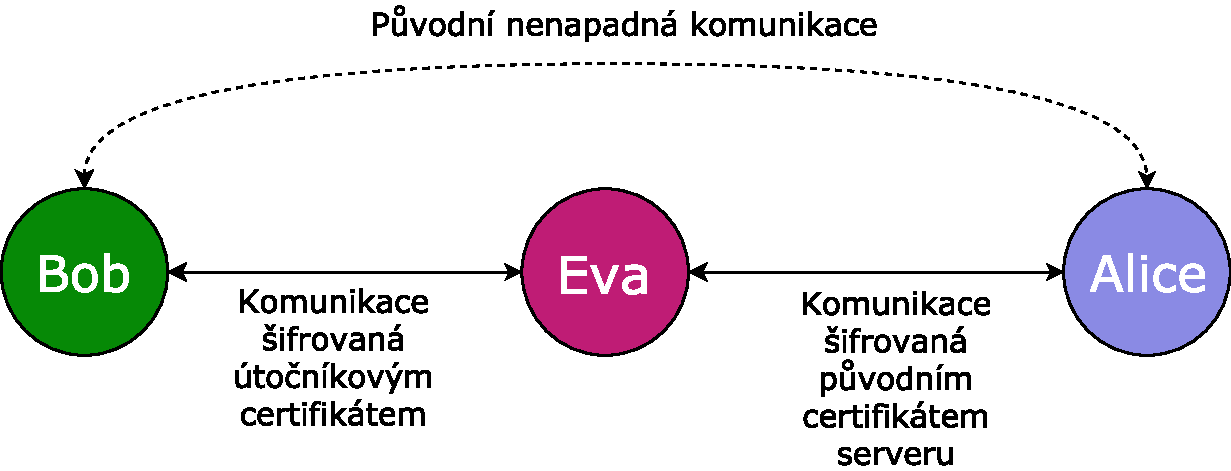
\includegraphics[width=\textwidth]{images/mitm.pdf}
    \caption[\textit{Man-in-the-middle} útok]{\textit{Man-in-the-middle} útok. Eva funguje jako nežádoucí prostředník mezi Bobem (klientem) a Alicí (původním serverem). Díky tomu má přístup ke zprávám obou účastníků komunikace. \cite{mitm}}
    \label{fig:mitm}
\end{figure}

\section{\textit{Hashování}}

\textit{Hashováním} se obecně rozumí vytvoření otistku pevné délky -- \textit{hashe} -- z~libovolných vstupních dat. Důležitou vlastností je jednosměrnost tohoto procesu, tedy že z~vytvořeného otisku již nelze zrekonstruovat původní vstup. \cite{hash_crackstation}

V~této práci je \textit{hashování} použito při ukládání hesel. Heslo uložené v~čitelné podobě není při úniku souboru s~heslem nijak chráněno. Proto je vhodné uložit místo hesla samotného jeho \textit{hash}. Pokud dojde k~úniku \textit{hashovaných} hesel, je pro útočníka velmi problematické  získat z~otisků čitelná hesla \cite{hash_crackstation}.

\textit{Hashování} lze provést pomocí mnoha algortimů, ne všechny se však hodí k~zabezpečení ukládaných hesel. Některé algoritmy, jako například MD5 či SHA-1, nejsou dostatečně výpočetně náročné, takže umožňují efektivní útoky hrubou silou (lze dostatečně rychle spočítat všechny možné kombinace vstupů do dané délky a tím zjistit jaký vstup odpovídá danému \textit{hashi}) \cite{hash_crackstation}. 

Pro bezpečné ukládání hesel je tedy nutné použít dostatečné náročný algoritmus. V~této práci je použit algoritmus Bcrypt, který je považován za vhodný k~\textit{hashování} uložených hesel \cite{hash_crackstation}.

\subsection{Solení \textit{hashů}}

\textit{Hashování} hesla je vhodné doplnit o~proces takzvaného \uv{solení}. Při něm se nevytváří otisk samotného hesla, ale hesla doplněného o~náhodně vygenerovaný řetězec -- sůl. To ztěžuje použítí předpočítaných tabulek (například tabulky s~otisky často používaných hesel) pro útoky hrubou silou \cite{hash_crackstation}.

Pro bližší informace o~bezpečném ukládání hesel doporučuji článek \textit{Salted Password Hashing - Doing it Right} \cite{hash_crackstation}.
